\documentclass[12pt,a4paper]{article}

% ===== Codificación y español =====
\usepackage[utf8]{inputenc}
\usepackage[T1]{fontenc}
\usepackage[spanish, es-tabla]{babel}

% ===== Márgenes y gráficos =====
\usepackage{geometry}
\geometry{margin=2.5cm}
\usepackage{graphicx}
\usepackage{float}        % [H] para fijar figuras/tablas
\usepackage{subcaption}   % subfiguras
\usepackage{booktabs}     % tablas más bonitas
\usepackage{amsmath}

% ===== Hipervínculos y referencias =====
\usepackage{hyperref}
\hypersetup{
  colorlinks=true,
  linkcolor=black,
  citecolor=black,
  urlcolor=blue
}

\usepackage{siunitx}
\sisetup{
  output-decimal-marker = {.}, % decimal con punto
  group-separator = {,},       % miles con coma
  group-minimum-digits = 4,
  group-digits = integer,
  table-number-alignment = center,
  round-mode = places,
  detect-all = true            % ignora configuraciones de babel
}

% Ayuda al manejo de tablas
\usepackage{tabularx}
\usepackage{adjustbox}
\usepackage{longtable}

% cleveref mejora \ref: escribe "Figura 1", "Tabla 2", etc.
\usepackage[capitalise,noabbrev]{cleveref}

% Ajuste de nombres en cleveref
\crefname{figure}{figura}{figuras}
\Crefname{figure}{Figura}{Figuras}
\crefname{subfigure}{subfigura}{subfiguras}
\Crefname{subfigure}{Subfigura}{Subfiguras}
\crefname{table}{tabla}{tablas}
\Crefname{table}{Tabla}{Tablas}
\crefname{equation}{ecuación}{ecuaciones}
\Crefname{equation}{Ecuación}{Ecuaciones}
\crefname{section}{sección}{secciones}
\Crefname{section}{Sección}{Secciones}

% Listas más controlables
\usepackage{enumitem}

\graphicspath{{figuras/}}

% ===== Título y autoría =====
\title{\textbf{Proyecto Final Big Data: Módulo No Supervisado}}
\author{Haessler Joan Ortiz Moncada \\[0.5cm]
        Universidad Distrital Francisco José de Caldas \\
        Facultad de Ingeniería \\
        Curso: Big Data}
\date{\today}

\begin{document}

\maketitle

\section{Introducción}
Este documento presenta el desarrollo de los ejercicios del \texttt{Taller\_7} del curso de 
Big Data, documentando los hallazgos y los análisis correspondientes. El taller se centra en 
el archivo \texttt{dato\_taller.mat} proporcionado por el docente, que contiene tres conjuntos 
de datos: (i) \texttt{x\_prueba}, una matriz de \(1000\times 20\); (ii) \texttt{x\_entena}, 
otra matriz de \(1000\times 20\); y (iii) \texttt{y\_prueba}, un vector de etiquetas de tamaño 
\(1000\times 1\) asociado a \texttt{x\_entena}. El objetivo es generar un vector de etiquetas 
para \texttt{x\_prueba} utilizando la información de \texttt{x\_entena} y su correspondiente 
vector de etiquetas \texttt{y\_prueba}, mediante las técnicas de agrupamiento no supervisado 
vistas en clase.

\section{Metodología}
Con la información proporcionada, se prepararon los datos en \texttt{MATLAB} —por tratarse de un 
archivo nativo— extrayendo la información de \texttt{dato\_taller.mat} y convirtiendo cada conjunto 
al formato \emph{CSV}, que luego se cargó en un \texttt{Jupyter Notebook} ejecutado en Google Colab; 
previo a aplicar los modelos, se verificó la naturaleza de los datos y el dominio de las características, 
y se realizó una selección de variables con el fin de mejorar el desempeño de los algoritmos; 
posteriormente, se implementaron y compararon varios modelos de agrupamiento no supervisado vistos en
clase —incluyendo \emph{k}-means, agrupamiento jerárquico, mapas autorganizados (SOM. por sus siglas en inglés) 
y DBSCAN— evaluando distintas configuraciones (hiperparámetros) para seleccionar las que ofrecieran mejores 
métricas de desempeño; el trabajo sigue el orden establecido en el \texttt{Taller\_7} y contó con la asistencia 
de la IA Gemini en parte del código; finalmente, el código, los datos utilizados y el informe pueden consultarse 
en la carpeta \texttt{taller\_7} del repositorio de GitHub \href{https://github.com/HaesslerOrtiz/bigdata}{\texttt{bigdata\_repositorio}}.

\section{Desarrollo}
\subsection{Descripción de los datos}
El archivo \texttt{dato\_taller.mat} es un archivo de \texttt{MATLAB} de tipo \emph{struct} que contiene 
tres campos: \texttt{x\_prueba}, \texttt{x\_entena} y \texttt{y\_prueba}. El primero es una matriz de tamaño 
\(10000\times 20\); el segundo, otra matriz de tamaño \(1000\times 20\); y el tercero, un vector de tamaño 
\(1000\times 1\) que contiene las etiquetas asociadas a las filas de \texttt{x\_entena}. En cuanto a los datos, 
no se proporciona información adicional sobre su origen, naturaleza o significado, ni sobre los nombres de las 
características. Respecto al dominio de las características, se observa que los valores de las columnas de 
\texttt{x\_prueba} y \texttt{x\_entena} se encuentran estandarizados y, como es lógico, son datos de tipo 
\emph{double} (precisión doble). El conjunto de datos \texttt{x\_entena} fue renombrado a \texttt{x\_entrena} 
para reflejar mejor su propósito en el contexto del taller. En cuanto al vector de etiquetas \texttt{y\_prueba}, 
se observó que tiene una clasifacación binaria, con valores de 1 y -1, y que está un poco desbalanceado 
(ver \cref{fig:dist_clase}), ya que 531 de las etiquetas son 1 y el restante son -1, es decir, 469. Por otra pate, 
ningún conjunto de datos contiene valores o registros nulos o faltantes.

\begin{figure}[H]
  \centering
  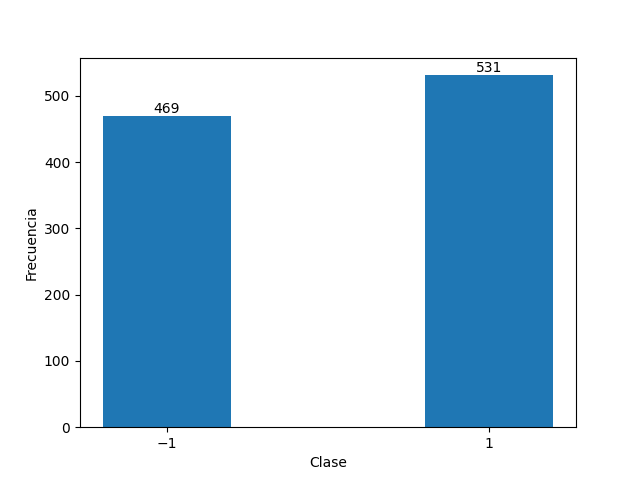
\includegraphics[width=0.8\textwidth]{dist_clase.png}
  \caption{Distribución de clases en \texttt{y\_prueba}.}
  \label{fig:dist_clase}
\end{figure}

\subsection{Preparación de los datos}
Antes de aplicar los modelos de agrupamiento, se unificaron los conjuntos \texttt{x\_entrena} y \texttt{x\_prueba} 
en un único conjunto denominado \texttt{x\_total}, con el fin de aprovechar toda la información disponible y 
facilitar la evaluación del desempeño del modelo propuesto. La unificación se realizó concatenando verticalmente 
ambas matrices, obteniéndose una matriz de tamaño \(11000\times 20\). Se asumió que las características de ambos 
conjuntos corresponden a las mismas variables. Dado que las características no estaban nombradas, se asignaron 
identificadores genéricos a las columnas de \texttt{x\_total}, desde \texttt{col1} hasta \texttt{col20}; para las 
etiquetas, el campo se denominó \texttt{clase}. Como paso previo a la selección de características, se llevó a 
cabo un filtrado de valores atípicos mediante el rango intercuartílico (\emph{IQR}). Se empleó un umbral de 
\(1.5\times \mathrm{IQR}\) para definir los límites superior e inferior y se eliminó todo registro cuyo valor en 
cualquiera de sus características quedara por fuera de dichos límites. Con este procedimiento se suprimieron \(1218\) 
registros, quedando \(9782\) observaciones en un nuevo conjunto denominado \texttt{x\_total\_filtrado}; el 
conjunto \texttt{x\_total} se conservó sin modificaciones. Este filtrado busca facilitar el agrupamiento en métodos 
que no modelan explícitamente \emph{outliers}, como \emph{k}-means y el agrupamiento jerárquico. Con esta reducción 
de muestras se pierde alrrededor del 12\% de la información original.

Otro aspecto analizado fue la distribución de los valores de las características (véase \cref{fig:variables_distribution}), 
con el fin de identificar posibles sesgos o la necesidad de aplicar transformaciones. De este examen se concluyó 
que no eran necesarias transformaciones adicionales, pues las variables presentan distribuciones aproximadamente 
simétricas respecto de su media y una curtosis "normal".

\begin{figure}[H]
  \centering
  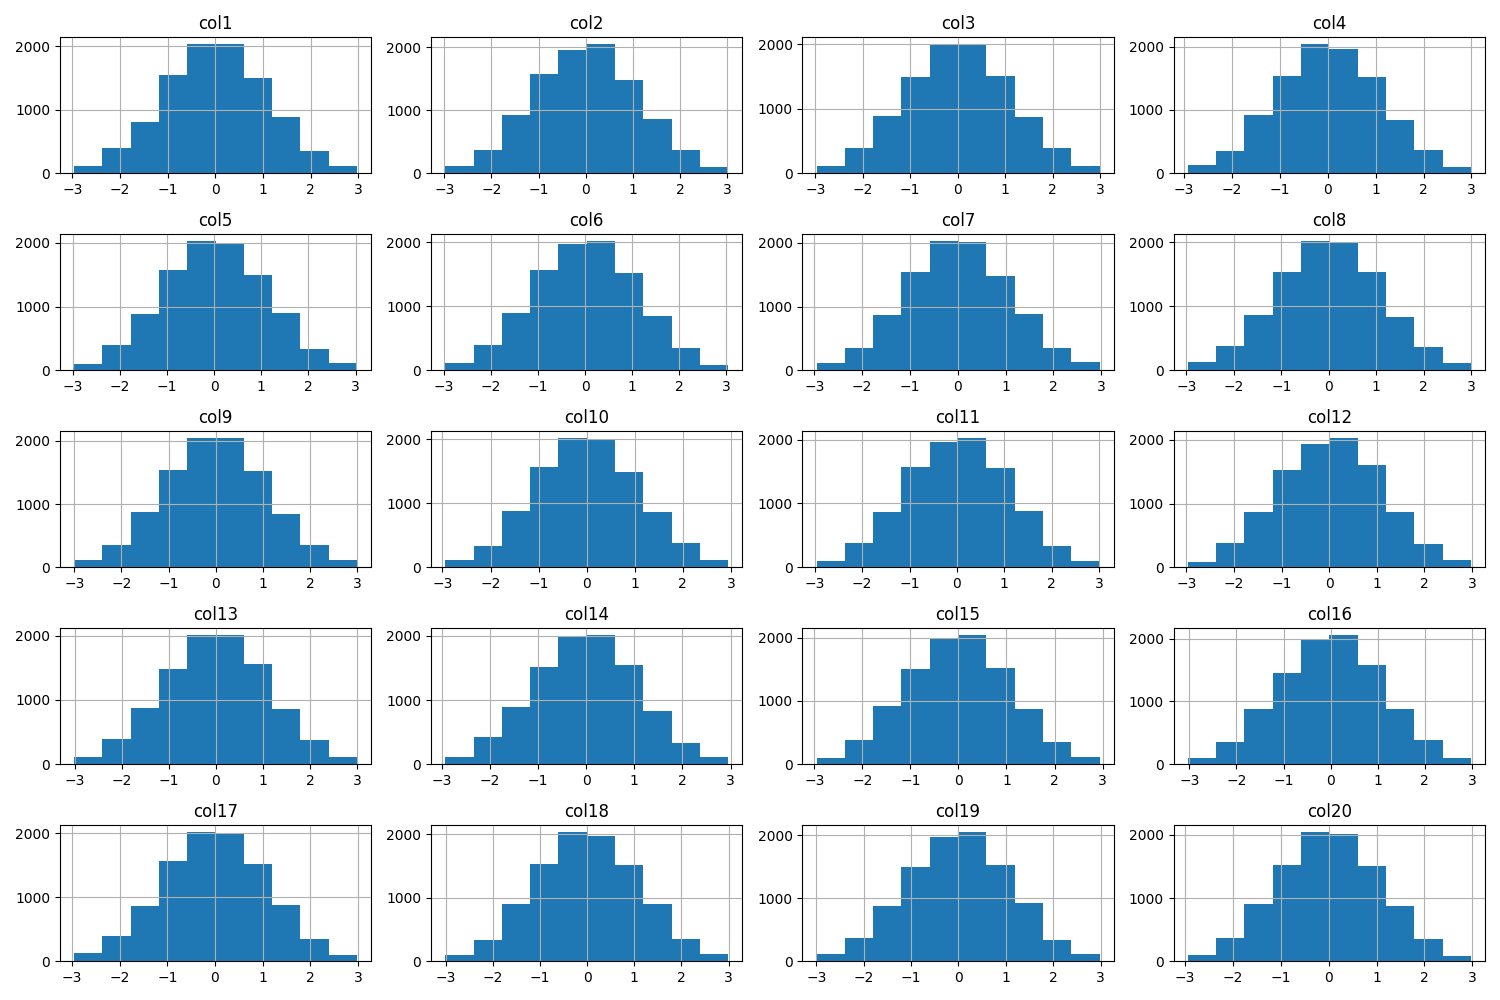
\includegraphics[width=0.9\textwidth]{variables_distribution.png}
  \caption{Distribución de las características.}
  \label{fig:variables_distribution}
\end{figure}

Al observar el gráfico anterior se podría teorizar que el conjunto de datos de estudio, corresponde a uno 
de naturaleza sintética y que guarda relación con alguna fígura geométrica.

\subsection{Selección de características}
Dado que no se proporciona información sobre el significado de las características, se optó por utilizar 
un análisis de correlación (correlación de Pearson) para identificar posibles relaciones lineales entre las 
características, además, también se implementó un análisis de componentes principales (\emph{PCA}, por sus sigla en 
inglés) para explorar la reducción de la dimensionalidad de los datos originales. 

Se calculó la matriz de correlación para las 20 características de \texttt{x\_total\_filtrado} y se visualizó mediante 
un mapa de calor (ver \cref{fig:correlacion}). Se observó que algunas todas las características tienen una correlación 
baja entre sí (valores cercanos a 0), lo que sugiere (\textit{a priori}) que no hay redundancia significativa entre 
ellas. Por lo tanto, el análisis de correlación no indicó la necesidad de eliminar ninguna característica.

\begin{figure}[H]
  \centering
  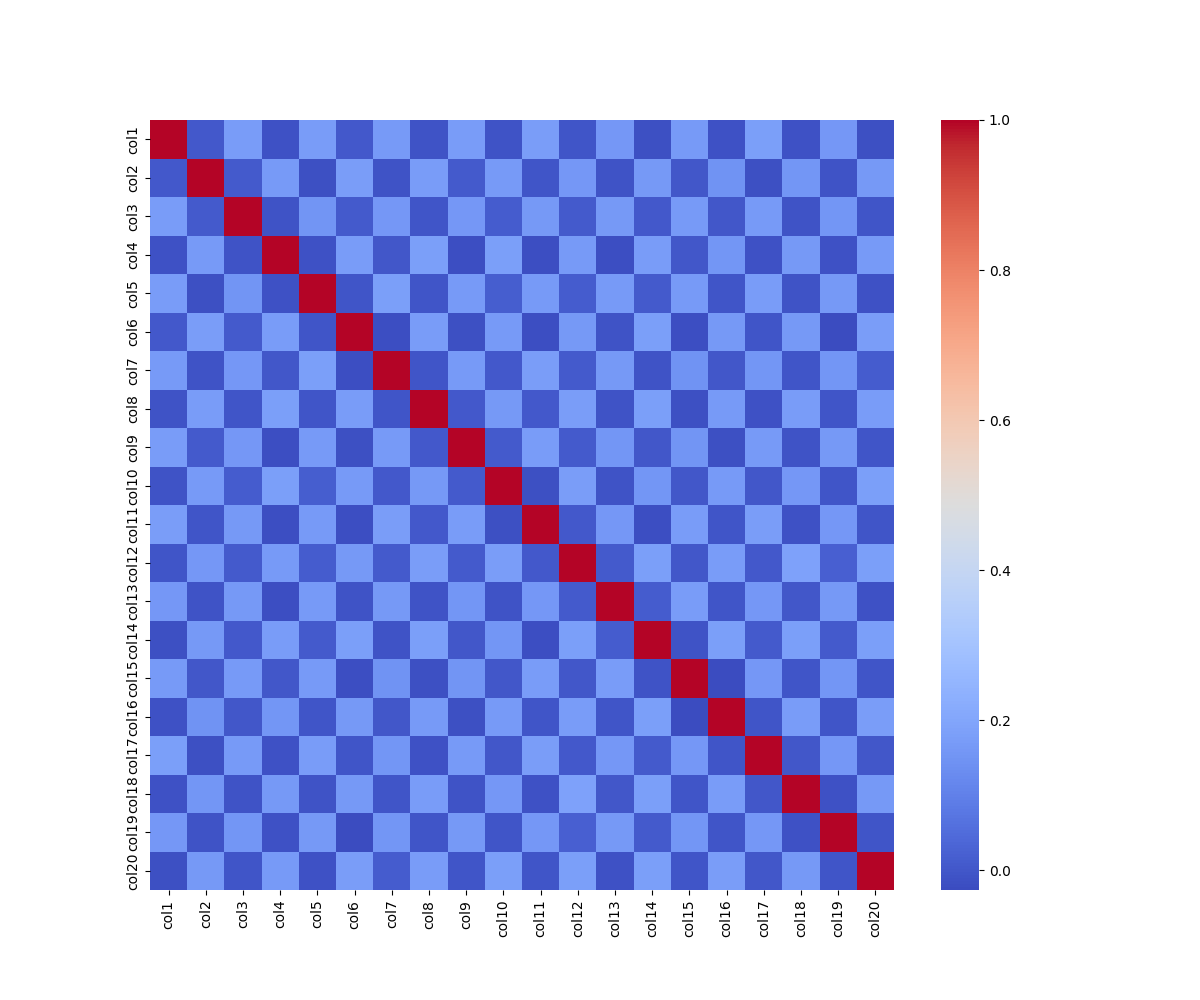
\includegraphics[width=0.9\textwidth]{correlacion_heatmap.png}
  \caption{Matriz de correlación entre las características de \texttt{x\_total}.}
  \label{fig:correlacion}
\end{figure}

Se aplicó \emph{PCA} a \texttt{x\_total} para evaluar la reducción de dimensionalidad. Se observó que las dos primeras 
componentes principales explican aproximadamente el \(25\%\) de la varianza total (esto es, cerca de \(12.5\%\) 
cada una; véase \cref{fig:pca}), mientras que las restantes presentan aportes pequeños y similares (alrededor de 
\(\sim 4\%\) cada una). Para este \emph{PCA} se consideró un umbral de varianza explicada del \(95\%\) para determinar el 
número óptimo de componentes a retener; se encontró que se requieren al menos \(19\) componentes para alcanzar 
dicho umbral, lo cual indica que la mayoría de las características originales contribuyen de forma significativa 
a la varianza total. En consecuencia, se decidió conservar todas las características originales para el análisis 
de agrupamiento, puesto que reducir a dos dimensiones implicaría una pérdida sustantiva de información. 

\begin{figure}[H]
  \centering
  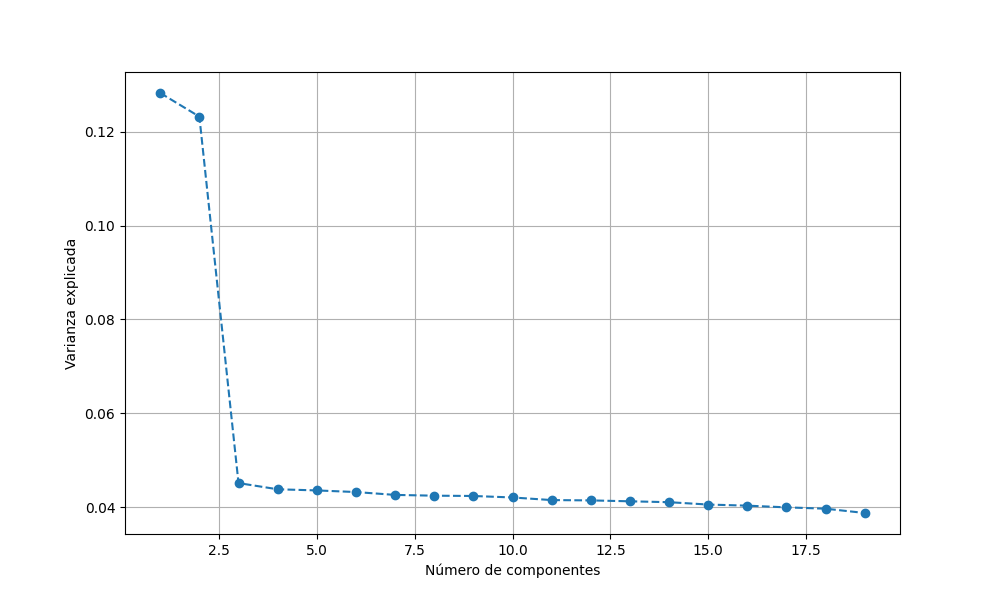
\includegraphics[width=0.9\textwidth]{pca_varianza.png}
  \caption{Varianza explicada por cada \emph{PCA}.}
  \label{fig:pca}
\end{figure}

La \cref{tab:pca_varianza} muestra la varianza explicada y la varianza acumulada para cada uno de los componentes 
principales generados.

\begin{table}[ht]
  \centering
  \begin{small}
    \begin{tabular}{rcc}
      \toprule
      \textbf{Componente} & \textbf{Varianza explicada} & \textbf{Varianza acumulada} \\
      \midrule
      1  & 12.82\% & 12.82\% \\
      2  & 12.32\% & 25.14\% \\
      3  & 4.51\%  & 29.66\% \\
      4  & 4.38\%  & 34.04\% \\
      5  & 4.36\%  & 38.40\% \\
      6  & 4.32\%  & 42.72\% \\
      7  & 4.26\%  & 46.98\% \\
      8  & 4.25\%  & 51.23\% \\
      9  & 4.24\%  & 55.47\% \\
      10 & 4.21\%  & 59.68\% \\
      11 & 4.15\%  & 63.83\% \\
      12 & 4.15\%  & 67.97\% \\
      13 & 4.13\%  & 72.10\% \\
      14 & 4.11\%  & 76.21\% \\
      15 & 4.06\%  & 80.26\% \\
      16 & 4.03\%  & 84.30\% \\
      17 & 4.00\%  & 88.29\% \\
      18 & 3.97\%  & 92.26\% \\
      19 & 3.88\%  & 96.14\% \\
      \bottomrule
    \end{tabular}
    \caption{\emph{PCA}: varianza explicada por componente y acumulada.}
    \label{tab:pca_varianza}
  \end{small}
\end{table}

\subsection{k-means}
Se entrenó un modelo de \emph{k}-means para distintos números de grupos, probando \(k\in[2,20]\). Para 
cada \(k\), los centroides iniciales se eligieron con la técnica \emph{k}-means++ y se realizaron 10 reinicios 
independientes para obtener la mejor solución. En cada reinicio, el \emph{algoritmo de Lloyd} 
iteró hasta 100 pasos como máximo o hasta que la función objetivo (inercia) dejara de mejorar más de 
\(10^{-4}\) entre iteraciones consecutivas. Se registró la mejor inercia final por cada \(k\) para 
construir el gráfico del codo (número de clusters vs. inercia) y, adicionalmente, se generó un gráficos 
\emph{Silhoutte} con el fin de comparar la calidad de la separación entre grupos y elegir el \(k\) que 
mejor organiza los datos. La \cref{fig:kmeans} muestra el resultado de este procedimiento.

\begin{figure}[H]
  \centering
  \begin{subfigure}{0.45\textwidth}
    \centering
    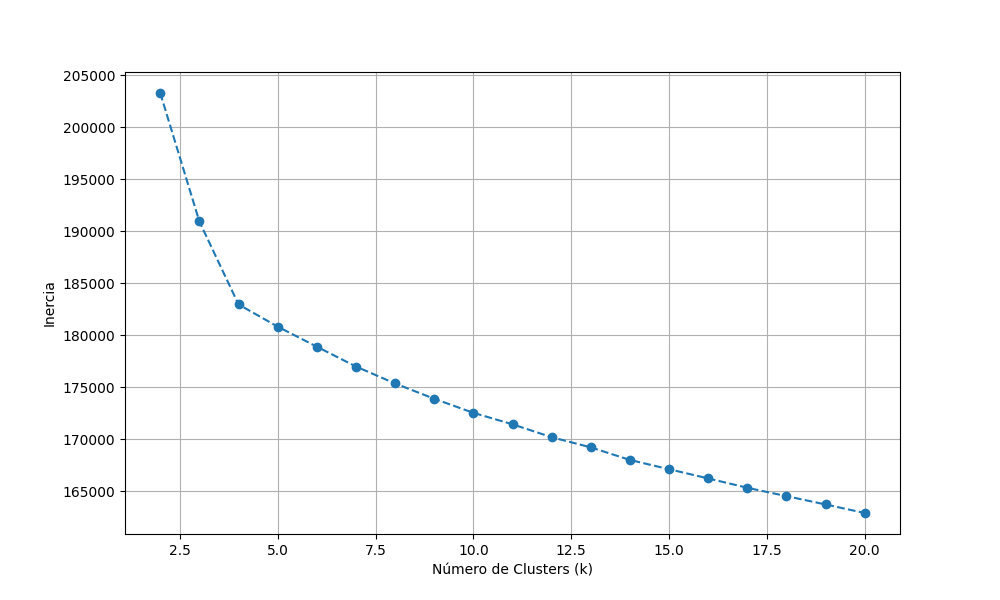
\includegraphics[width=\linewidth]{kmeans_elbow.png}
    \caption{Gráfico del codo.}
    \label{fig:kmeans_elbow}
  \end{subfigure}\hfill
  \begin{subfigure}{0.45\textwidth}
    \centering
    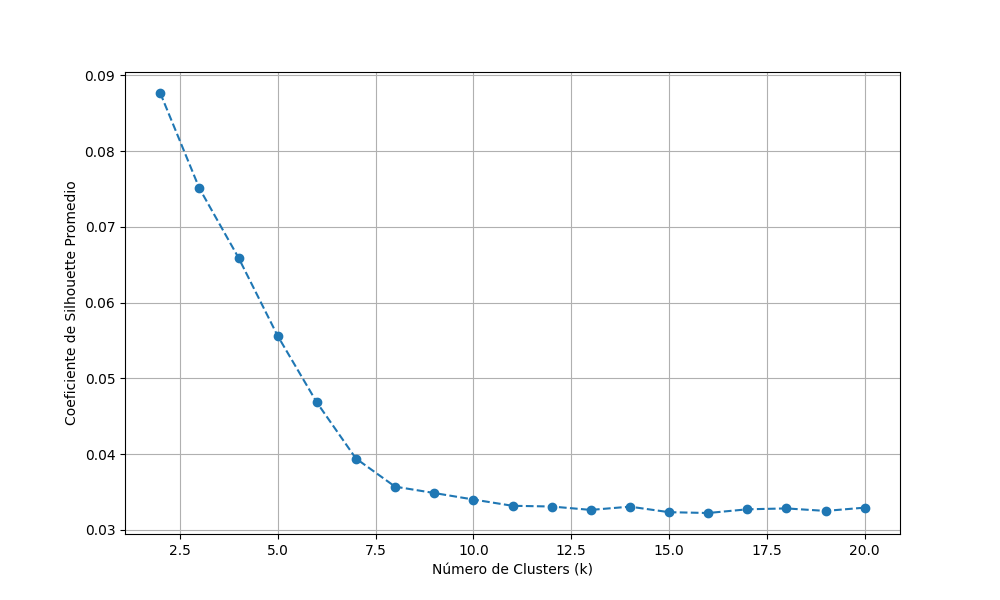
\includegraphics[width=\linewidth]{kmeans_silhouette.png}
    \caption{Gráfico de \emph{silhouette}.}
    \label{fig:kmeans_silhouette}
  \end{subfigure}
  \caption{Implementación de \emph{k}-means.}
  \label{fig:kmeans}
\end{figure}

De los resultados se concluye que la mejor relación entre reducción de inercia y número de grupos 
(sin caer en un exceso de grupos), según el gráfico del codo, se da aproximadamente para 
\(k=5\). Sin embargo, al observar el gráfico de \emph{silhouette}, aunque el mejor promedio del 
coeficiente (más cercano a 1) es cuando \(k=2\), se aprecian valores de \emph{silhouette} muy bajos, 
lo que indica una separación poco nítida entre grupos. En conjunto, estos hallazgos sugieren que 
\emph{k}-means no resulta un método adecuado de agrupamiento para este conjunto de datos.

\subsection{Agrupamiento jerárquico}
Para reducir el costo del agrupamiento jerárquico, primero se condensó el conjunto estandarizado 
(\(9782\times 20\)) en protoclústeres (\emph{m}) mediante \emph{Mini-Batch k-means}, que actualiza centroides 
con mini-lotes (subconjuntos de \(1024\)–\(2048\) filas por iteración) para acelerar el cálculo y 
disminuir el uso de memoria. Se probó un rango de tamaños \(m\in\{400,600,800,1000,1200\}\) con 
configuración reproducible para replicar los resultados, reinicios múltiples (\texttt{n\_init} = 10; 
varias inicializaciones y elección de la mejor por menor inercia/SSE) y un criterio de parada por 
tolerancia (\texttt{tol} = 1\texttt{e-4}) dentro de un límite de iteraciones 
(\texttt{max\_iter}\( \approx 100\)). El criterio de parada detiene el algoritmo cuando la inercia deja 
de mejorar de forma apreciable entre iteraciones (la caída es menor a la tolerancia). El rango de \(m\) equilibra 
detalle y costo: con \(n = 9782\), valores entre \(\sim4\times 10^{-2}n\) y \(\sim1.2\times 10^{-1}n\) 
(es decir, \(\approx 400\)–\(1200\)) mantienen el paso jerárquico en un coste \(\mathcal{O}(m^{2})\) manejable 
para los servidores de \emph{Colab}, esto permite prservar resolución suficiente para el dendrograma y evitan tanto 
microgrupos (si \(m\) es muy alto) como protoclústeres excesivamente grandes (si \(m\) es muy bajo); 
además, dejan tamaños esperados por protoclúster de \(n/m \approx 8\)–\(25\) observaciones, adecuados para 
representar la estructura sin sobrefragmentar. La \cref{fig:protocluster_silhouette} muestra como se comportan 
los mejores \emph{coeficiente de Silhouette} para cada uno de los \(m\) probados. 

\begin{figure}[H]
  \centering
  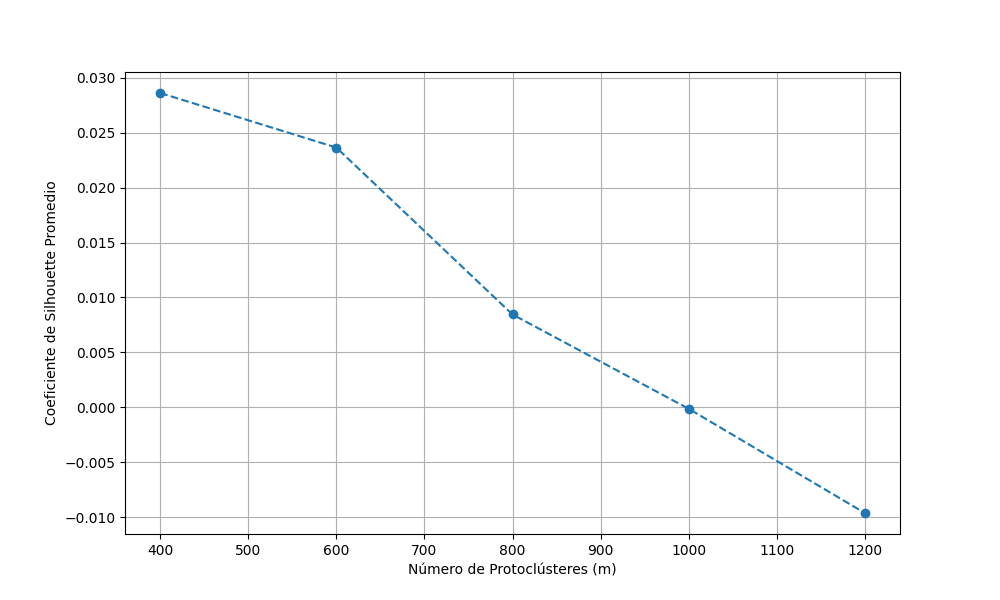
\includegraphics[width=0.9\textwidth]{protocluster_silhouette.png}
  \caption{\emph{Coeficiente de Silhouette} versus \(m\). }
  \label{fig:protocluster_silhouette}
\end{figure}

Del gráfico anterior se observa que, con \(m = 400\), se obtiene el mayor \emph{coeficiente de silhouette}, 
aunque sin alcanzar valores altos, esto no resulta preocupante en esta etapa, pues se trata de un paso 
previo al agrupamiento jerárquico.

Con la anterior información, se tomaron los centroides de los protoclústeres (\(m\) = 400) para trabajar con un resumen 
del conjunto y así agilizar el cálculo. Con esos centroides se construyó el árbol jerárquico (dendrograma) probando 
los enlaces \emph{ward, single, average y complete}. Luego, para cada método, se cortó el árbol en distintos números 
de grupos (\(k\) de 2 a 12) y esas etiquetas se propagaron a todas las filas originales (cada fila hereda la etiqueta 
del protoclúster al que pertenece). Con esas etiquetas completas se calculó el \emph{coeficiente de Silhouette} para medir 
qué tan bien se separan los grupos, y se guardó el mejor valor por cada método. Finalmente, para cada método se generó un 
dendrograma simplificado (mostrando solo los últimos 100 grupos) que ilustra visualmente la partición seleccionada. Como 
dato curioso, los mejores valores de \emph{Silhouette} fueron con \(k = 2\), al igual que cuando se desarrolló el 
método de agrupamiento \emph{k-means}. Los dendrogramas generados se muestran en la \cref{fig:dendrogramas}.

\begin{figure}[H]
  \centering

  % --- Fila superior ---
  \begin{subfigure}{0.48\textwidth}
    \centering
    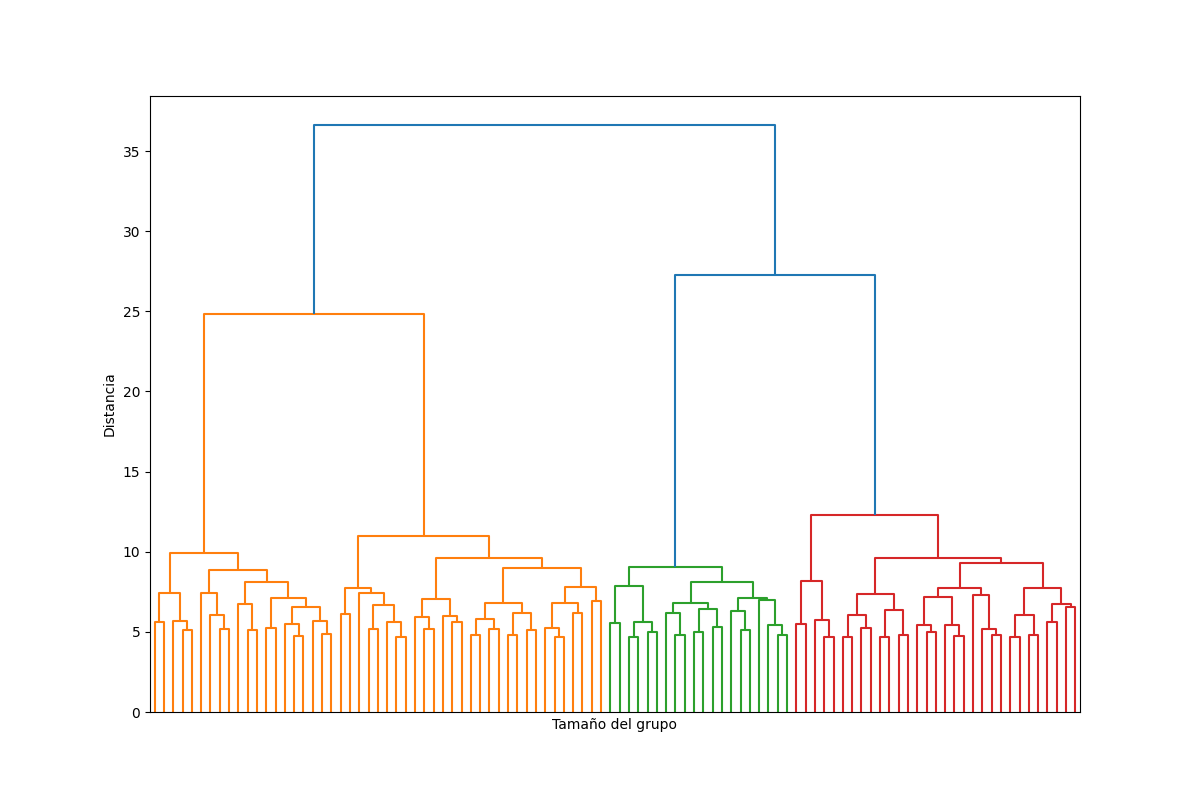
\includegraphics[width=\linewidth]{dendro_ward_best.png}
    \caption{Enlace \emph{ward} con \(k = 2\).}
    \label{fig:ward}
  \end{subfigure}\hfill
  \begin{subfigure}{0.48\textwidth}
    \centering
    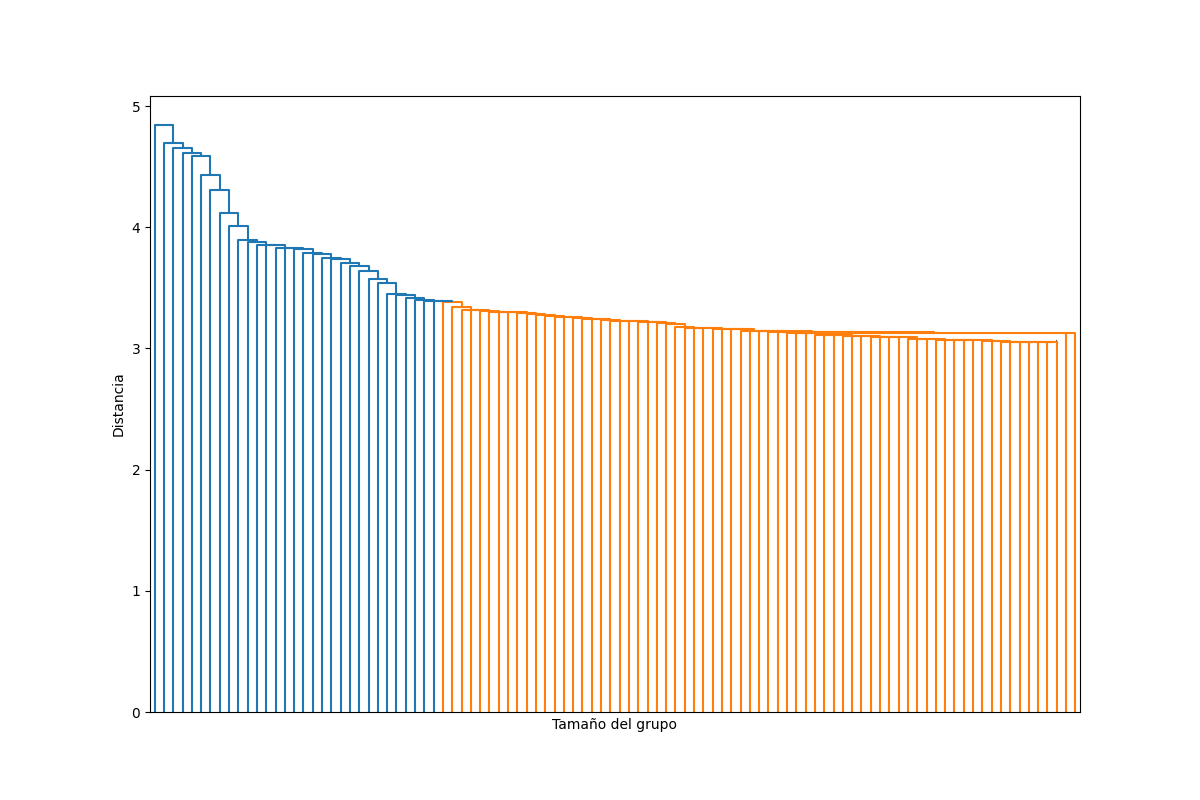
\includegraphics[width=\linewidth]{dendro_single_best.png}
    \caption{Enlace \emph{single} con \(k = 2\).}
    \label{fig:single}
  \end{subfigure}

  \par\medskip % separación entre filas

  % --- Fila inferior ---
  \begin{subfigure}{0.48\textwidth}
    \centering
    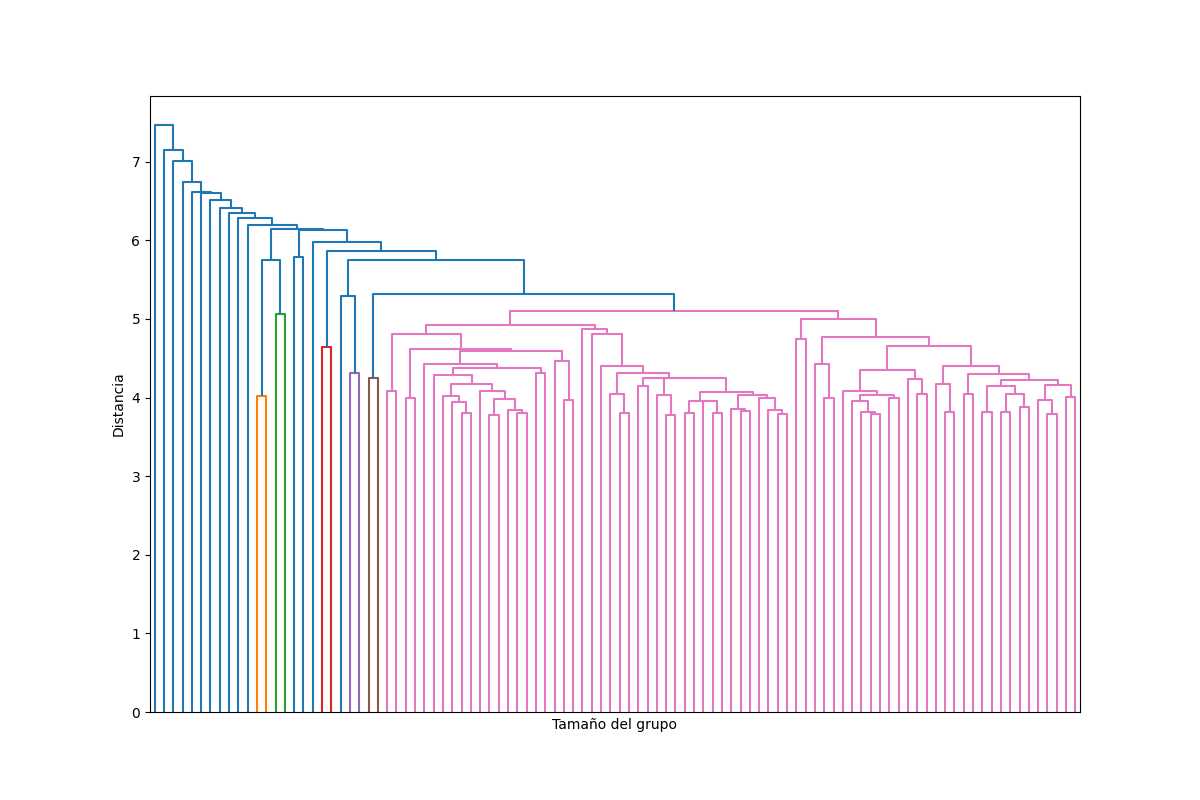
\includegraphics[width=\linewidth]{dendro_average_best.png}
    \caption{Enlace \emph{average} con \(k = 2\).}
    \label{fig:average}
  \end{subfigure}\hfill
  \begin{subfigure}{0.48\textwidth}
    \centering
    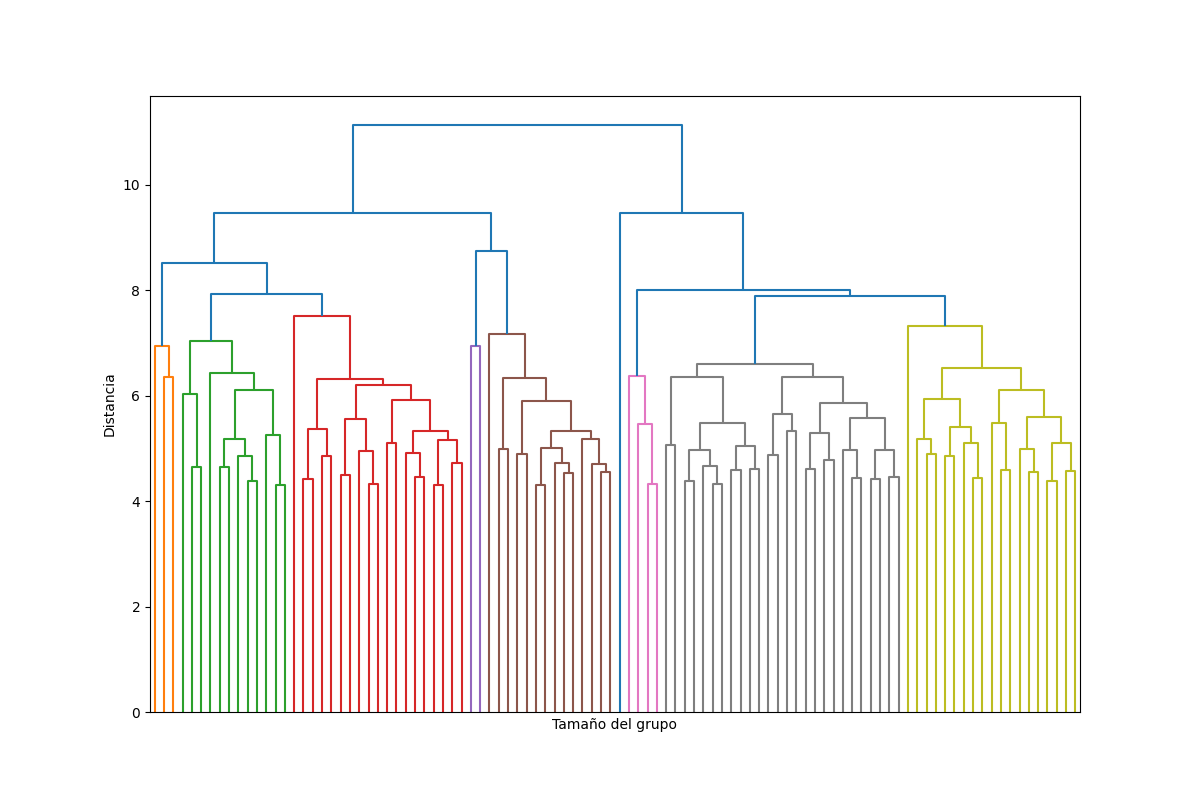
\includegraphics[width=\linewidth]{dendro_complete_best.png}
    \caption{Enlace \emph{complete} con \(k = 2\).}
    \label{fig:complete}
  \end{subfigure}

  \caption{Dendrogramas de los mejores agrupamientos encontrados.}
  \label{fig:dendrogramas}
\end{figure}

A grandes rasgos, los cuatro dendrogramas se comportan como se esperaría según el criterio de enlace: el 
\emph{single} muestra el típico “encadenamiento” (fusiones muy bajas y uno que otro salto al final), 
\emph{complete} arma grupos más compactos y deja ver cortes razonables en \(k\approx 3\)–\(5\); 
\emph{average} queda en un punto medio, con separación moderada; y \emph{ward} es el que luce más 
“limpio”, con saltos finales marcados y tamaños más equilibrados, sugiriendo cortes naturales en 
\(k\approx 2\)–\(4\). Sin embargo, los correspondientes valores de \emph{Silhouette}, arrojan valores bajos, 
lo que significa que la separación alcanzada no es buena, lo que permite concluir que los agrupamientos 
jerárquicos implementados no resultan adecuados para este conjunto de datos. La \cref{tab:best_jerarquico} 
muestra las configuraciones para los agrupamientos con los mejores valores de \emph{Silhouette}.

\begin{table}[ht]
  \centering
  \begin{small}
    \begin{tabular}{lcc}
      \toprule
      \textbf{Método} & \textbf{\(k\)} & \textbf{Silhouette} \\
      \midrule
      Ward     & 2 & 0.0725 \\
      Single   & 2 & 0.0867 \\
      Average  & 2 & 0.1569 \\
      Complete & 2 & 0.0700 \\
      \bottomrule
    \end{tabular}
    \caption{\emph{Silhouette} por método de enlace.}
    \label{tab:best_jerarquico}
  \end{small}
\end{table}

\subsection{DBSCAN}
El método de agrupamiento \emph{DBSCAN} requiere definir dos parámetros: el radio de vecindad 
(\(\varepsilon\)) y el número mínimo de vecinos (\texttt{min\_samples}). Para estimar \(\varepsilon\), 
se generó la curva de distancias al \(k\)-ésimo vecino (\emph{k-distance}) probando 
\(\texttt{min\_samples}\in\{5,8,10,12\}\), con el fin de ubicar el “codo” donde la distancia al 
\(k\)-ésimo vecino se dispara y, así, aproximar la escala a la que los datos se agrupan. La 
\cref{fig:kdist_plot} muestra los resultados de esta búsqueda.

\begin{figure}[H]
  \centering

  % --- Fila superior ---
  \begin{subfigure}{0.48\textwidth}
    \centering
    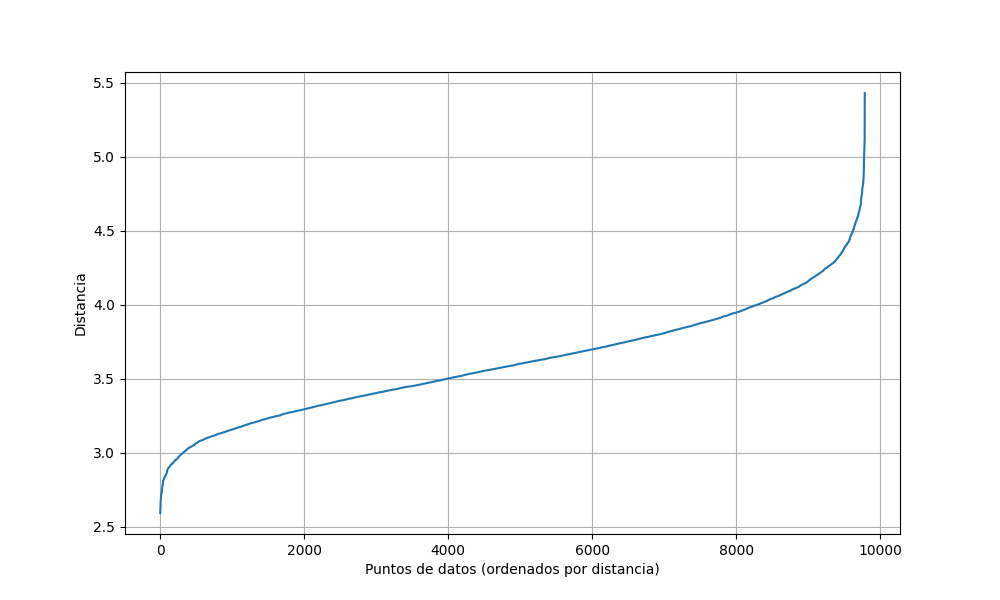
\includegraphics[width=\linewidth]{kdist_plot_min_samples_5.png}
    \caption{Distancia al k-esimo vecino (5).}
    \label{fig:kplot_kdist5}
  \end{subfigure}\hfill
  \begin{subfigure}{0.48\textwidth}
    \centering
    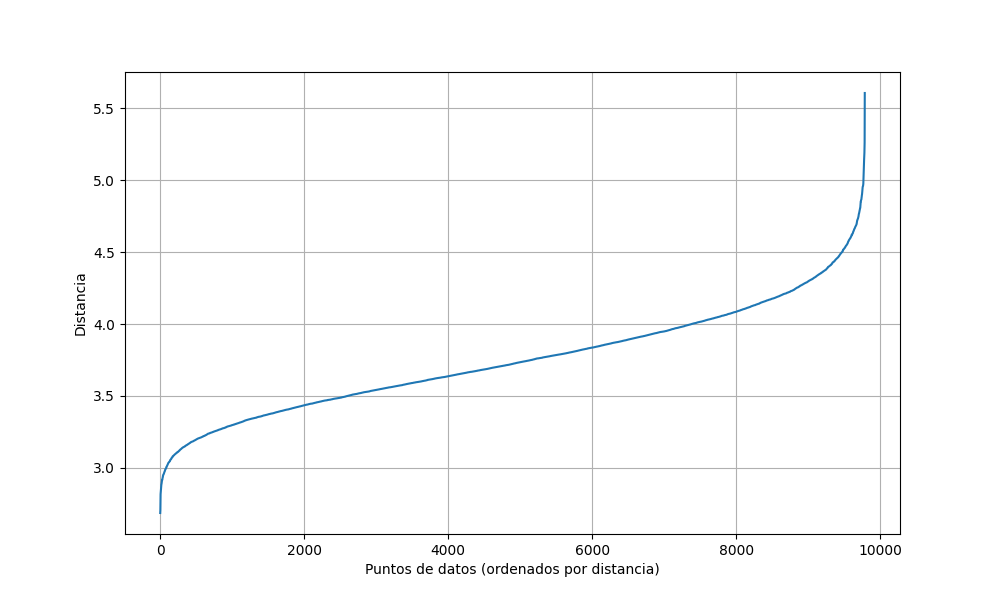
\includegraphics[width=\linewidth]{kdist_plot_min_samples_8.png}
    \caption{Distancia al k-esimo vecino (8).}
    \label{fig:kplot_kdist8}
  \end{subfigure}

  \par\medskip % separación entre filas

  % --- Fila inferior ---
  \begin{subfigure}{0.48\textwidth}
    \centering
    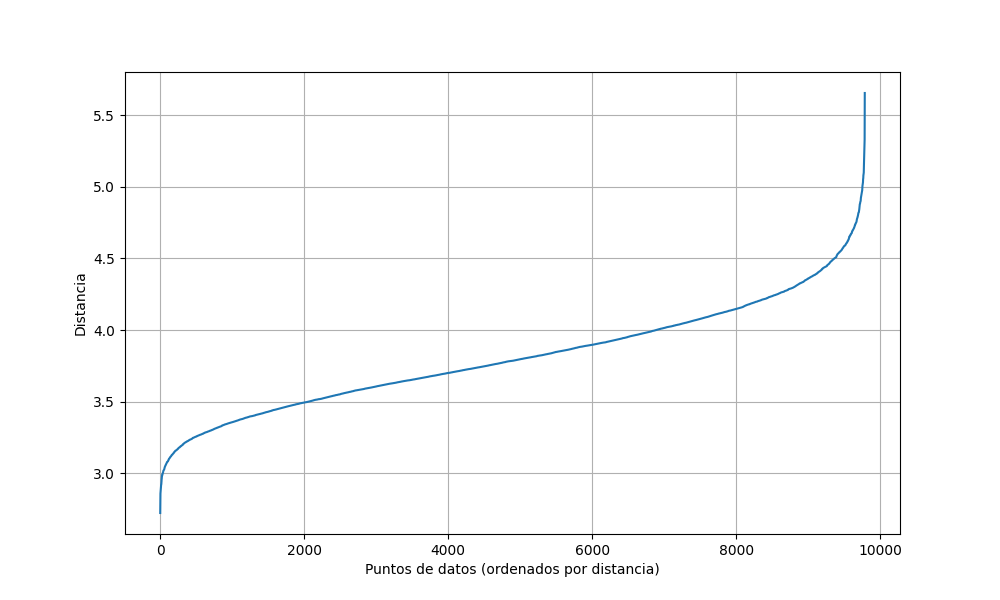
\includegraphics[width=\linewidth]{kdist_plot_min_samples_10.png}
    \caption{Distancia al k-esimo vecino (10).}
    \label{fig:kplot_kdist10}
  \end{subfigure}\hfill
  \begin{subfigure}{0.48\textwidth}
    \centering
    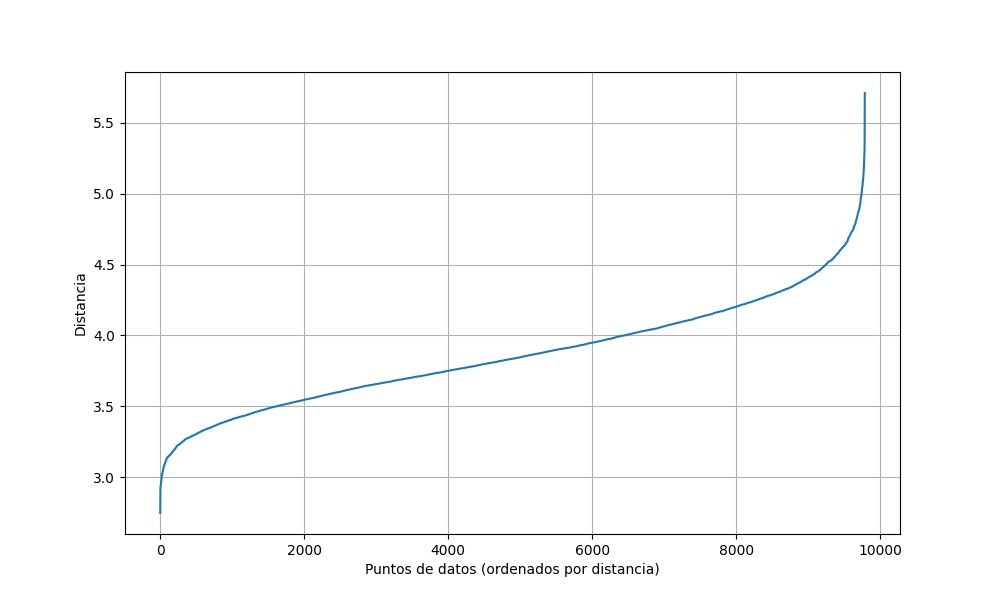
\includegraphics[width=\linewidth]{kdist_plot_min_samples_12.png}
    \caption{Distancia al k-esimo vecino (12).}
    \label{fig:kplot_kdist12}
  \end{subfigure}

  \caption{Gráficos para identificar \(\varepsilon\).}
  \label{fig:kdist_plot}
\end{figure}

Con base en el gráfico anterior, la distancia al \(k\)-ésimo vecino presenta un incremento marcado 
en el rango [4.5 - 5.0]. A partir de ello, se definió una rejilla para \(\varepsilon\) con paso 
de 0.1 y se mantuvieron inicialmente los valores de \texttt{min\_samples} \(\{5,8,12\}\) para evaluar 
\emph{DBSCAN}. No obstante, el algoritmo no logró separar adecuadamente el conjunto: con distancia euclidiana 
y radios amplios, casi todos los puntos quedaron en un único grupo (lo que impide calcular \emph{silhouette}); 
al reducir el radio y aumentar \texttt{min\_samples}, el comportamiento fue similar. Con distancia de 
\emph{coseno}, ajustando finamente \(\varepsilon\), se obtuvieron dos grupos, pero con frontera difusa y 
un \emph{silhouette} cercano a cero; al exigir mayor densidad, las métricas mejoraron a costa de etiquetar 
gran parte de los datos como “ruido”, lo cual resulta poco útil. En síntesis, en el espacio original de 20 
variables \emph{DBSCAN} no identifica “islas” de densidad bien definidas.

\subsection{SOM: Mapas autorganizados}
Utilizando el conjunto de datos \texttt{x\_total\_filtrado}, se entrenó un SOM con vecindad gaussiana en dos 
fases (ordenamiento global y ajuste fino) y se evaluó un barrido focalizado de cinco retículas (\(18\times 18\), 
\(22\times 22\), \(26\times 26\), \(30\times 30\) y \(34\times 34\)), seleccionando el modelo por 
\emph{Quantization Error} (QE) (ver \cref{fig:qe_grid}). Se obtuvo el mejor resultado con \(30\times 30\) neuronas (QE \(\approx 4.072\)), 
muy próximo a \(32\times 32\) (QE \(\approx 4.075\)) y \(34\times 34\) (QE \(\approx 4.076\)), lo que sugiere que 
un buen ajuste sucede en \(30\pm 2\). Para interpretar la magnitud del \emph{QE}, se contrastó con una referencia 
geométrica propia de datos estandarizados (\emph{z}-score): en \(d=20\) dimensiones, la escala natural viene dada 
por \(\sqrt{d}=\sqrt{20}\approx 4.47\); por tanto, el \emph{QE} alcanzado está por debajo de dicha escala. La 
\emph{U-Matrix} (ver \cref{fig:umatrix1}) del \(30\times 30\) evidenció fronteras bien definidas y zonas internas 
homogéneas, coherentes con un mapa ordenado. En síntesis, se logró un equilibrio adecuado entre detalle y costo 
computacional, y el barrido reducido permitió acortar tiempos sin comprometer la calidad, contextualizando el 
\emph{QE} con una métrica comprensible (\(\sqrt{d}\) y \(\mathrm{NQE}=\mathrm{QE}/\sqrt{d}\)) en lugar de tomar 
su valor absoluto sin referencia.

\begin{figure}[H]
  \centering
  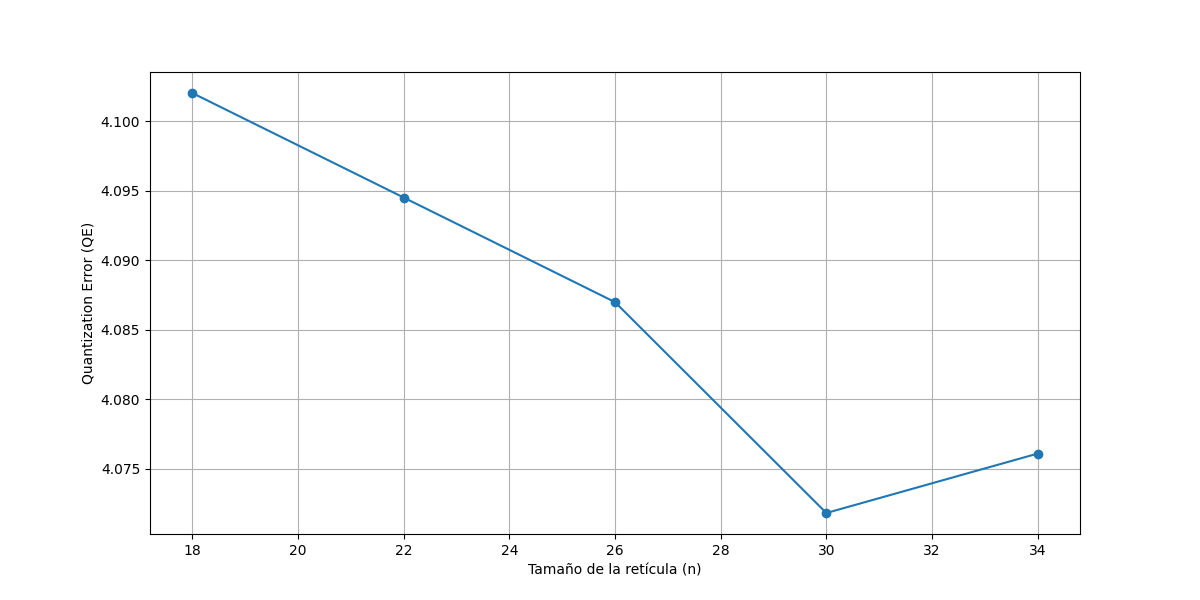
\includegraphics[width=0.9\textwidth]{som_qe_vs_grid_size.png}
  \caption{\emph{QE} versus tamaño de retícula.}
  \label{fig:qe_grid}
\end{figure}

\paragraph*{Conclusión de la exploración actual.}
Como conclusión hasta el momento, los enfoques de agrupamiento tradicionales probados (\emph{k}-means, \emph{DBSCAN} y jerárquico) 
arrojaron valores bajos y/o inestables de \emph{Silhouette}, lo que sugiere separaciones poco nítidas entre grupos. En 
contraste, el \emph{SOM} mostró un desempeño más prometedor. En resumen, dentro del conjunto de pruebas no 
supervisadas realizadas hasta este punto, el \emph{SOM} constituye la alternativa más sólida para estructurar el 
espacio de datos de estudio.

La siguiente labor del presente informe consiste en retomar los mejores modelos de esta exploración 
para evaluarlos no solo sobre el conjunto de datos utilizado hasta ahora, sino también sobre subespacios de componentes principales; 
allí se incorporarán métricas supervisadas (p.\,ej., desempeño de clasificación en el subconjunto etiquetado) con el fin de elegir 
el modelo que mejor agrupe y ofrezca mayor capacidad de clasificación.

\begin{figure}[H]
  \centering
  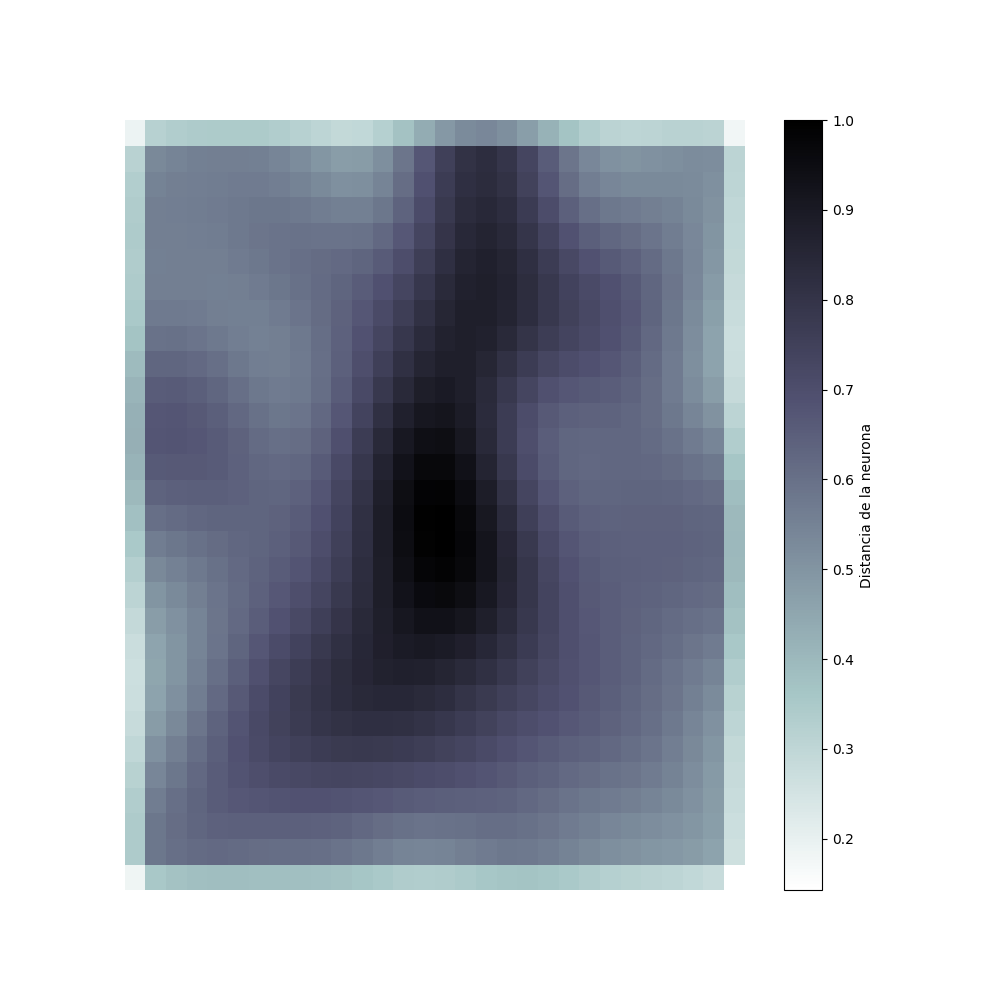
\includegraphics[width=0.9\textwidth]{umatrix_som_30x30.png}
  \caption{\emph{U-Matrix} mejor retícula según \emph{QE}. }
  \label{fig:umatrix1}
\end{figure}

\subsection{Análisis semisupervisado}
En esta sección se retoman los mejores modelos de agrupamiento no supervisado probados previamente, con la intención de 
etiquetar los grupos formados a partir de las etiquetas conocidas de \texttt{y\_prueba} y evaluar su desempeño en términos 
de clasificación. Se emplearon los conjuntos \texttt{x\_total\_filtrado} y \texttt{combined\_x\_PCA\_df}; este último corresponde 
a la transformación por \emph{PCA} de las 20 dimensiones originales. No obstante, para el desarrollo de los modelos se trabajó 
con 15 componentes principales (aprox.\ 80\% de varianza explicada), a fin de contrastar si \emph{PCA} mejora el agrupamiento 
sin perder demasiada información. A continuación se describen los resultados por modelo.

\subsubsection{\emph{k}-means}
Se entrenaron modelos de \emph{k}-means con \(k\in\{2,3,4,5\}\) tanto en el conjunto original como en el transformado por 
\emph{PCA}. Se revaluaron el coeficiente de \emph{silhouette} y el gráfico del codo para cada \(k\). Como era esperable, el 
mejor \emph{silhouette} promedio se obtuvo con \(k=2\), aunque con valores bajos; el gráfico del codo mostró una reducción 
marcada de la inercia al aumentar \(k\), con un codo en torno a \(k=4\), comportamiento consistente en ambos conjuntos. Para 
la evaluación supervisada, se asignaron etiquetas a los grupos por mayoría y se calcularon matriz de confusión, precisión y 
exactitud. La \cref{fig:kmeans_final} muestra las matrices de confusión para \(k=2\) en ambos conjuntos.

\begin{figure}[H]
  \centering
  \begin{subfigure}{0.45\textwidth}
    \centering
    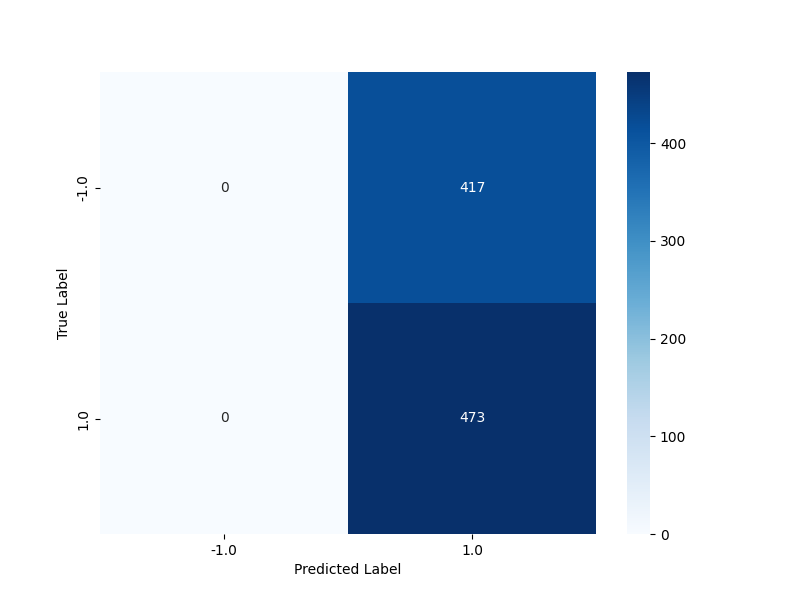
\includegraphics[width=\linewidth]{kmeans_confusion_final.png}
    \caption{\texttt{x\_total\_filtrado}.}
    \label{fig:kmeans_confusion_final_xfiltrado}
  \end{subfigure}\hfill
  \begin{subfigure}{0.45\textwidth}
    \centering
    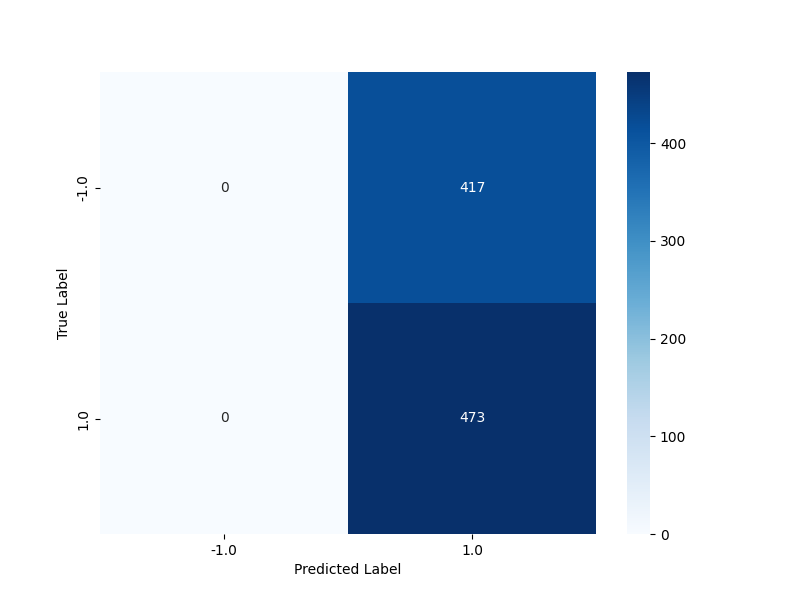
\includegraphics[width=\linewidth]{kmeans_confusion_final.png}
    \caption{\texttt{combined\_x\_PCA\_df}.}
    \label{fig:kmeans_confusion_final_PCA}
  \end{subfigure}
  \caption{Matrices de confusión para \emph{k}-means con \(k=2\).}
  \label{fig:kmeans_final}
\end{figure}

Como se observa en el gráfico anterior, ambos modelos de \emph{k}-means producen clasificaciones idénticas: el 
conjunto transformado por \emph{PCA} no muestra mejoras frente al conjunto original. La exactitud global es baja 
porque el clasificador asigna todos los datos etiquetados a una sola clase (1). En consecuencia, recupera 
correctamente todos los ejemplos de la clase 1 (recall \(=1\)), pero comete todos los falsos positivos sobre la 
clase \(-1\). Cabe aclarar, que el número de datos clasificados no llega a 1000, pues algunos puntos quedaron fuera 
del conjunto tras el filtrado por \emph{IQR}.

\subsubsection{Agrupamiento jerárquico}
Se repitió el procedimiento de agrupamiento jerárquico sobre \texttt{x\_total\_filtrado} y \texttt{combined\_x\_PCA\_df}, 
utilizando los criterios de enlace \emph{ward} y \emph{average}. Aunque el análisis preliminar sugería \(k=2\) como valor 
óptimo por \emph{silhouette}, se evaluó \(k\in\{2,\dots,6\}\) para observar el comportamiento, dado que los dendrogramas 
indicaban posibles cortes en \(k=3\)–\(5\). Como antes, se asignaron etiquetas por mayoría y se calcularon las métricas 
de clasificación (precisión, exactitud y matriz de confusión). Aun cuando los valores de \emph{silhouette} fueron bajos, 
el desempeño en clasificación mejoró al incrementar \(k\); a partir de \(k=4\)–\(6\) ya no hubo mejoras adicionales ni 
cambios en la asignación, por lo que se eligió \(k=4\) como configuración final, pese a mantener \emph{silhouette} 
bajo. En todas las comparaciones, \texttt{x\_total\_filtrado} superó al conjunto transformado por \emph{PCA}, y el mejor 
enlace en ambos casos fue \emph{ward}. La \cref{fig:jerarquico_final} muestra las matrices de confusión para \(k=4\) en 
ambos conjuntos.

\begin{figure}[H]
  \centering
  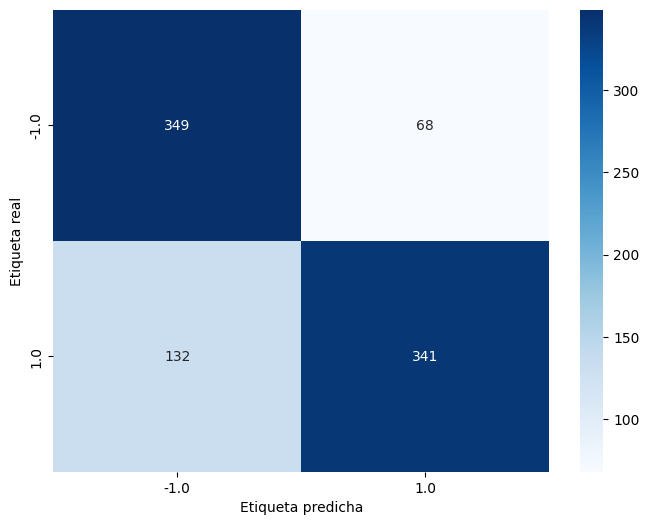
\includegraphics[width=0.8\textwidth]{jerarquico_final.png}
  \caption{Matriz de confusión mejor modelo de agrupación jerarquico. }
  \label{fig:jerarquico_final}
\end{figure}

El modelo jerárquico sobre \texttt{x\_total\_filtrado}, con enlace \emph{ward} y \(k=4\), presenta falsos positivos 
en ambas clases particularmente en la clase \(-1\), pero aun así alcanza métricas de clasificación satisfactorias, 
como se muestra en la \cref{tab:jerarquico_metrics}.

\begin{table}[ht]
  \centering
  \begin{small}
    \begin{tabular}{lr}
      \toprule
      \textbf{Métrica} & \textbf{Valor} \\
      \midrule
      Silhouette & 0.0442 \\
      Exactitud (Accuracy) & 0.7753 \\
      Precisión (Macro) & 0.7797 \\
      Exactitud clase \(-1\) & 0.8369 \\
      Exactitud clase \(1\) & 0.7209 \\
      \bottomrule
    \end{tabular}
  \end{small}
  \caption{Agrupamiento jerárquico (\emph{ward}) con \(k=4\): métricas de desempeño.}
  \label{tab:jerarquico_metrics}
\end{table}

\subsubsection{DBSCAN}
De acuerdo con la exploración inicial, \emph{DBSCAN} no separó adecuadamente los datos en el espacio 
original de 20 dimensiones. Al repetir el procedimiento sobre \verb|combined_x_pca_df|, se exploró 
$\varepsilon\in[4.5,5.0]$ y \texttt{min\_samples} $\in\{5,8,10,12,16\}$, incluyendo valores más altos 
para forzar grupos más densos, así como la distancia de coseno. Sin embargo, los resultados no 
mejoraron: se obtuvo nuevamente un único \emph{cluster}, lo que impide calcular el coeficiente de 
\emph{silhouette} y, como era de esperarse, el desempeño en clasificación equivale a asignar todas las 
muestras a la clase mayoritaria (1). Cabe aclarar que también se probó \emph{DBSCAN} sobre 
\verb|x_total_filtrado| y variando $\varepsilon$, sin mejoras: se seguía obteniendo un solo \emph{cluster} 
o, en su defecto, la mayoría de las muestras quedaban marcadas como ruido.

\subsubsection{SOM: Mapa autorganizado}
En cuanto al \emph{SOM}, se retomó el modelo entrenado con retícula $30\times 30$ sobre los conjuntos 
que se han venido trabajando en esta sección. Las neuronas se etiquetaron por \emph{voto mayoritario} 
con base en las muestras etiquetadas que mapeó cada BMU, y luego se evaluó la clasificación en el subconjunto 
etiquetado. Como se vaticinó en la exploración inicial, el método de agrupamiento basado en \emph{SOM} resultó 
en el que mejor desempeño de clasificación alcanzó, superando a los demás modelos, especificamente con el 
conjunto \texttt{combined\_x\_PCA\_df}. La \cref{fig:som_final} muestra la matriz de confusión obtenida.

\begin{figure}[H]
  \centering
  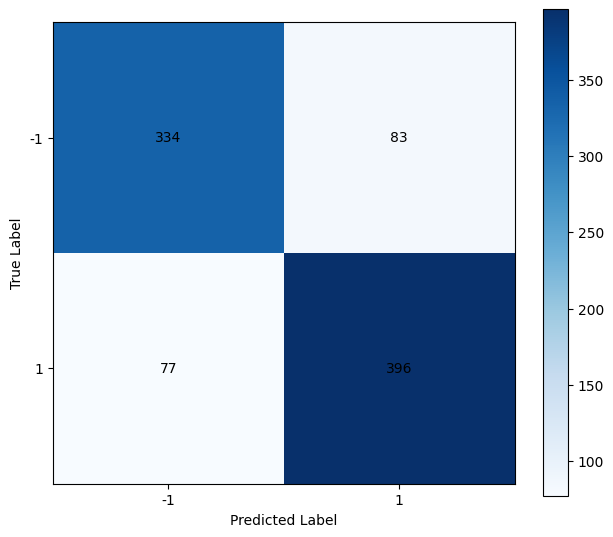
\includegraphics[width=0.8\textwidth]{SOM_final.png}
  \caption{Matriz de confusión mejor modelo \emph{SOM}. }
  \label{fig:som_final}
\end{figure}

Este modelo de agrupación basado en \emph{SOM} alcanzó métricas de clasificación satisfactorias, como 
se muestra en la \cref{tab:som_metrics}. 

\begin{table}[ht]
  \centering
  \begin{small}
    \begin{tabular}{lr}
      \toprule
      \textbf{Métrica} & \textbf{Valor} \\
      \midrule
      Exactitud (Accuracy)     & 0.8202 \\
      Precisión (Macro)        & 0.8197 \\
      Recall (Macro)           & 0.8191 \\
      F1 (Macro)               & 0.8193 \\
      Exactitud balanceada     & 0.8191 \\
      Exactitud clase \(-1\)   & 0.8010 \\
      Exactitud clase \(1\)    & 0.8372 \\
      \bottomrule
    \end{tabular}
  \end{small}
\caption{Métricas de desempeño mejor modelo \emph{SOM}.}
\label{tab:som_metrics}
\end{table}


\section{Entregable}
De acuerdo con el análisis realizado, se selecciona el modelo de agrupamiento basado en \emph{SOM} como 
el más representativo del conjunto de datos, utilizando como variables de entrada las 15 primeras 
componentes principales obtenidas por \emph{PCA}. Como entregable, se genera el vector de etiquetas para 
todo el conjunto \texttt{x\_prueba}, asignadas por el modelo seleccionado; este archivo es de tipo \emph{CSV} 
y corresponde a un vector columna de tamaño \(1\times 10000\) (una etiqueta por registro). Sin embargo, y para 
mayor claridad, se incluye también la matriz \texttt{x\_prueba} junto con sus etiquetas asignadas, resultando 
en un archivo \emph{CSV} de tamaño \(10000\times 21\) (\(20\) variables \(+\) \(1\) etiqueta), con el fin de 
evitar problemas de correspondencia entre archivos. El vector y la matriz se llaman respectivamente 
\texttt{som\_etiquetas.csv} y \texttt{x\_prueba\_som\_etiquetas.csv}.

\section{Conclusiones}

\begin{enumerate}
  \item El conjunto de datos analizado presenta una estructura que dificulta la tarea de agrupamiento. Las causas 
  pueden ser múltiples: desde la naturaleza intrínseca de las observaciones y la falta de información contextual 
  sobre las variables, hasta posibles sesgos en el conjunto etiquetado que no reflejan fielmente la estructura latente.

  \item Es posible que las clases del conjunto etiquetado hayan sesgado los análisis y la propuesta de modelos de 
  agrupamiento. De hecho, en la fase de exploración los mejores resultados se obtuvieron con \(k=2\), incluso en el 
  análisis de \emph{PCA}, se observó que las dos primeras componentes eran las de mayor aporte relativo. En otras 
  palabras, el hecho de observar dos clases y de que la exploración favoreciera \(k=2\) pudo llevar a asumir quizá de 
  forma indebida que existen dos grupos “naturales” en los datos, cuando podría no ser así.

  \item El análisis de correlación indicó que las variables no exhiben relaciones lineales fuertes entre sí, lo 
  que sugiere baja redundancia. En consecuencia, la reducción de dimensionalidad mediante \emph{PCA} puede no resultar  
  especialmente ventajosa en todos los casos, pues puede conllevar pérdida de información relevante. Sin embargo, en este 
  estudio, el uso de \emph{PCA} contribuyó a mejorar el desempeño de clasificación del modelo basado en \emph{SOM}.

  \item El agrupamiento jerárquico mostró que, al aumentar el número de grupos \(k\), mejoraba el desempeño en 
  clasificación; esto sugiere que también pudo haberse explorado un \(k\) mayor en la fase supervisada con 
  \emph{\(k\)-means}. Sin embargo, con las herramientas disponibles (gráfico del codo e índice de \emph{silhouette}) 
  no es posible establecer \emph{a priori} si el conjunto de datos contiene realmente más de dos grupos, teniendo en cuenta 
  la alta dimensionalidad del ocnjunto de datos que se trabajó.

  \item En general, los modelos de agrupamiento no supervisado tradicionales probados no lograron separar claramente los datos, lo que 
  se refleja especialmente en los bajos valores de \emph{silhouette} obtenidos. No obstante, al evaluar el desempeño 
  supervisado, algunos modelos (especialmente el jerárquico con \(k=4\)) alcanzaron métricas de clasificación aceptables, 
  lo que sugiere que las métricas de agrupamiento no supervisado no siempre reflejan el potencial de clasificación de 
  los modelos, es importante no desechar un modelo únicamente por sus bajos valores de \emph{silhouette}.

\end{enumerate}








\end{document}